\chapter{Теоретическая часть}
\section{Надёжность технических систем}

	Техническая система --- объект, представляющий собой множество взаимосвязанных элементов, рассматриваемых в определённом контексте как единое целое и отделённых от окружающей среды.
	
	Технический элемент --- объект, для которого в рамках данного рассмотрения не выделяются составные части.
	
	Структурная схема надёжности (ССН) --- логическое и графическое представление объекта, отображающее, каким образом безотказность его блоков и их сочетаний влияют на безотказность объекта. 

	ССН представляет собой условную запись работоспособного состояния системы через работоспособность элементов этой системы. ССН может быть задана:
	\begin{enumerate}
		\item аналитически;
		\item графически. 
	\end{enumerate}
	ССН должна:
	\begin{enumerate}
		\item иметь физический смысл;
		\item достаточно просто описывать работоспособность системы; 
		\item поддаваться алгоритмизации. 
	\end{enumerate}
	Виды ССН: 
	\begin{enumerate}
		\item ССН с основным соединением элементов (с последовательным соединением); 
		\item ССН с резервным соединением элементов (присутствуют резервирующие элементы).
	\end{enumerate}
\section{Надёжность технической системы с основным соединением элементов (без восстановления)}
	Аналитически ССН для такой системы задаётся следующим образом: отказ любого элемента системы влечёт за собой отказ системы. ССН основного соединения показана на рис.~\ref{img:20-0}
	\begin{figure}[h]
	  \centering
	  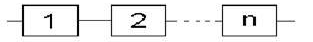
\includegraphics[width=.5\linewidth]{assets/connect}
	  \caption{CCН основного соединения}
	  \label{img:20-0}
	\end{figure}

	При условии независимости отказов элементов в системе (поток отказов без последствий) ВБР системы с основным соединением будет равна произведению ВБР её элементов:
	\begin{equation}
		P_{sys}(t) = \prod\limits_{i = 1}^{n}P_{i}(t).
	\end{equation}

	Если интенсивность отказов не постоянна, тогда:
	\begin{gather}
		P_{sys}(t) = e^{-\sum\limits_{i = 1}^{n}\;\int\limits_{0}^{t}\lambda_{i}(\tau)d\tau};\\
		T_{1,sys} = \int\limits_{0}^{\infty}P_{sys}(t)dt.
	\end{gather}

	Если интенсивность отказов постоянна, тогда:
	\begin{gather}
		P_{sys}(t) = e^{-\sum\limits_{i = 1}^{n}\lambda_{i}t};\\
		T_{1,sys} = \int\limits_{0}^{\infty}P_{sys}(t)dt;\\
		f_{sys}(t) = -\frac{d P_{sys}(t)}{d t} = \sum\limits_{i = 1}^{n}\lambda_{i}e^{-\sum\limits_{i = 1}^{n}\lambda_{i}t};\\
		\lambda_{sys} = \frac{P_{sys}(t)}{f_{sys}(t)} = \sum\limits_{i = 1}^{n}\lambda_{i}.
	\end{gather}

	Основные свойства системы с основным соединением элементов без восстановления: 
	\begin{enumerate}
		\item C увеличением количества элементов системы надёжность системы уменьшается; 
		\item Надёжность системы в целом заведомо ниже надёжности любого элемента системы;
		\item Устойчивость экспоненциального закона надёжности.
	\end{enumerate}

